\chapter{\label{chap:results}Resultados}

Para os cenários de teste definidos na Seção \ref{tab:cenarios} foram realizadas
simulações. Os resultados são apresentados a seguir.

\section{Cenário \textit{Low-rise}}

A Listagem \ref{lst:config:lowrise} exibe um excerto do arquivo de configuração
que define o cenário \textit{Low-rise}. A Tabela \ref{tab:results:lowrise}
mostra os resultados\footnote{Destacados encontram-se os melhores resultados
obtidos para cada métrica.} obtidos após a simulação.

\begin{listing}[htb!]
  \centering
    \begin{minted}[linenos,fontsize=\small]{yaml}
  # ...
  - name: Low-rise
    duration: 43200 # unidades de tempo
    scheduler: [ 0, 1 ] # simple, planning
    planningHorizon: 5
    cost_function: [ 0, 1, 2, 3 ] # randon, nn, bnn, weighted
    seed: 54TH7hboAG1iOsDIDhJp
    elevators: 2
    capacity: 2
    floors: [ 60, 520, 360, 360, 360, 240, 240, 240, 90, 90, 90 ]
  # ...
    \end{minted}
  \caption{Configuração do cenário \textit{Low-rise}.}
  \label{lst:config:lowrise}
\end{listing}

\begin{table}[htb!]
\centering
\caption{Resultados para o cenário \textit{Low-rise}.}
\label{tab:results:lowrise}
\begin{tabular}{|l|r|r|r|r|r|r|}
\hline
\multicolumn{1}{|c|}{\textbf{}} & \multicolumn{3}{c|}{\textbf{Tempo de Espera}} & \multicolumn{3}{c|}{\textbf{Tempo de Jornada}} \\ \hline
\textbf{Estratégia} & \multicolumn{1}{c|}{\textit{Médio}} & \multicolumn{1}{c|}{\textit{Desvio}} & \multicolumn{1}{c|}{\textit{Total}} & \multicolumn{1}{c|}{\textit{Médio}} & \multicolumn{1}{c|}{\textit{Desvio}} & \multicolumn{1}{c|}{\textit{Total}} \\ \hline
\textit{Simple / Random}   & 5.4064        & 4.1792        & 16933       & 4.4949        & 2.8676        & 14078        \\ \hline
\textit{Simple / NN}       & 3.5144        & 3.5768        & 11007       & 4.4700        & 2.8565        & 14000        \\ \hline
\textit{Simple / BNN}      & 3.3547        & 3.2931        & 10507       & \green 4.4674 & 2.9163        & \green 13992 \\ \hline
\textit{Simple / Weighted} & 3.7149        & 3.8036        & 11635       & 4.4719        & \green 2.7997 & 14006        \\ \hline
\textit{Planning}          & \green 3.1731 & \green 2.9171 & \green 9938 & 4.4770        & 3.0009        & 14022        \\ \hline
\end{tabular}
\end{table}

O \textit{tempo de espera médio} do \textit{planning} foi apenas $5.41\%$ melhor
em relação ao segundo colocado (\textit{better nearest neighbour}). Entretanto,
somado ao fato do \textit{desvio padrão} ter sido $12\%$ melhor, é uma forte
indicação de que \textit{planning} é a melhor estratégia para este cenário.

\begin{figure}[htb!]
  \centering
  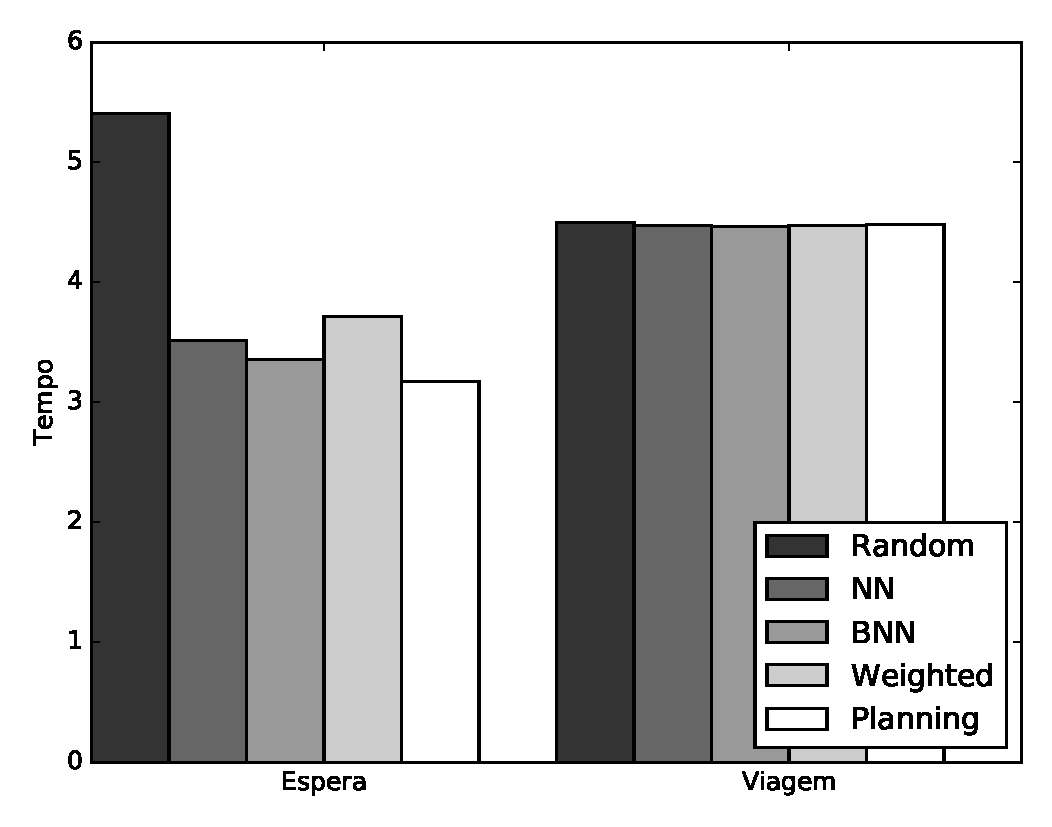
\includegraphics[scale=0.6]{img/low-rise-average-times-chart}
  \caption{Gráfico de resultados para o cenário \textit{Low-rise}.}
  \label{fig:result:average:low-rise}
\end{figure}

\section{Cenário \textit{High-rise}}
A Listagem \ref{lst:config:highrise} exibe um excerto do arquivo de configuração
que define o cenário \textit{High-rise}. A Tabela \ref{tab:results:highrise}
mostra os resultados\footnote{Destacados encontram-se os melhores resultados
obtidos para cada métrica.} obtidos após a simulação.

\begin{listing}[htb!]
  \centering
    \begin{minted}[linenos,fontsize=\small]{yaml}
  # ...
  - name: High-rise
    duration: 43200 # unidades de tempo
    scheduler: [ 0, 1 ]
    planningHorizon: 2
    cost_function: [ 0, 1, 2, 3 ]
    seed: w9JwgykwejtoL2icSgHo
    elevators: 8
    capacity: 10
    floors: [ 60, 520, 520, 520, 360, 360, 360, 360, 360, 360, 360, 360, 360,
             360, 360, 360, 360, 360, 360, 360, 360, 360, 360, 360, 360, 360,
             360, 360, 240, 240, 240, 240, 240, 240,  90,  90,  90,  90,  90 ]
  # ...
    \end{minted}
  \caption{Configuração do cenário \textit{High-rise}.}
  \label{lst:config:highrise}
\end{listing}

\begin{table}[htb!]
\centering
\caption{Resultados para o cenário \textit{High-rise}.}
\label{tab:results:highrise}
\begin{tabular}{|l|r|r|r|r|r|r|}
\hline
\multicolumn{1}{|c|}{\textbf{}} & \multicolumn{3}{c|}{\textbf{Tempo de Espera}} & \multicolumn{3}{c|}{\textbf{Tempo de Jornada}} \\ \hline
\textbf{Estratégia} & \multicolumn{1}{c|}{\textit{Médio}} & \multicolumn{1}{c|}{\textit{Desvio}} & \multicolumn{1}{c|}{\textit{Total}} & \multicolumn{1}{c|}{\textit{Médio}} & \multicolumn{1}{c|}{\textit{Desvio}} & \multicolumn{1}{c|}{\textit{Total}} \\ \hline
\textit{Simple / Random}   & 25.9981       & 28.0464        & 190124        & 15.2595        & 14.9190        & 111593        \\ \hline
\textit{Simple / NN}       & 20.3395       & 37.1902        & 148743        & 15.0993        & 11.4479        & 110421        \\ \hline
\textit{Simple / BNN}      & 13.5243       & 23.5950        &  98903        & 15.0550        & \green 10.2476 & 110097        \\ \hline
\textit{Simple / Weighted} & 31.0373       & 54.5909        & 226976        & \green 14.9915 & 18.9700        & \green 109633 \\ \hline
\textit{Planning}          & \green 8.6901 & \green 16.2139 &  \green 63551 & 15.1627        & 12.0920        & 110885        \\ \hline
\end{tabular}
\end{table}

Em cenários maiores e com um maior número de clientes percorrendo o prédio, os
ganhos em se utilizar \textit{planning} ficam ainda mais evidentes. Neste
cenário, seu \textit{tempo de espera médio} foi $35.74\%$ melhor em relação ao
segundo colocado (\textit{better nearest neighbour}). Já o \textit{desvio padrão}
foi $31.28\%$ melhor.

\begin{figure}[htb!]
  \centering
  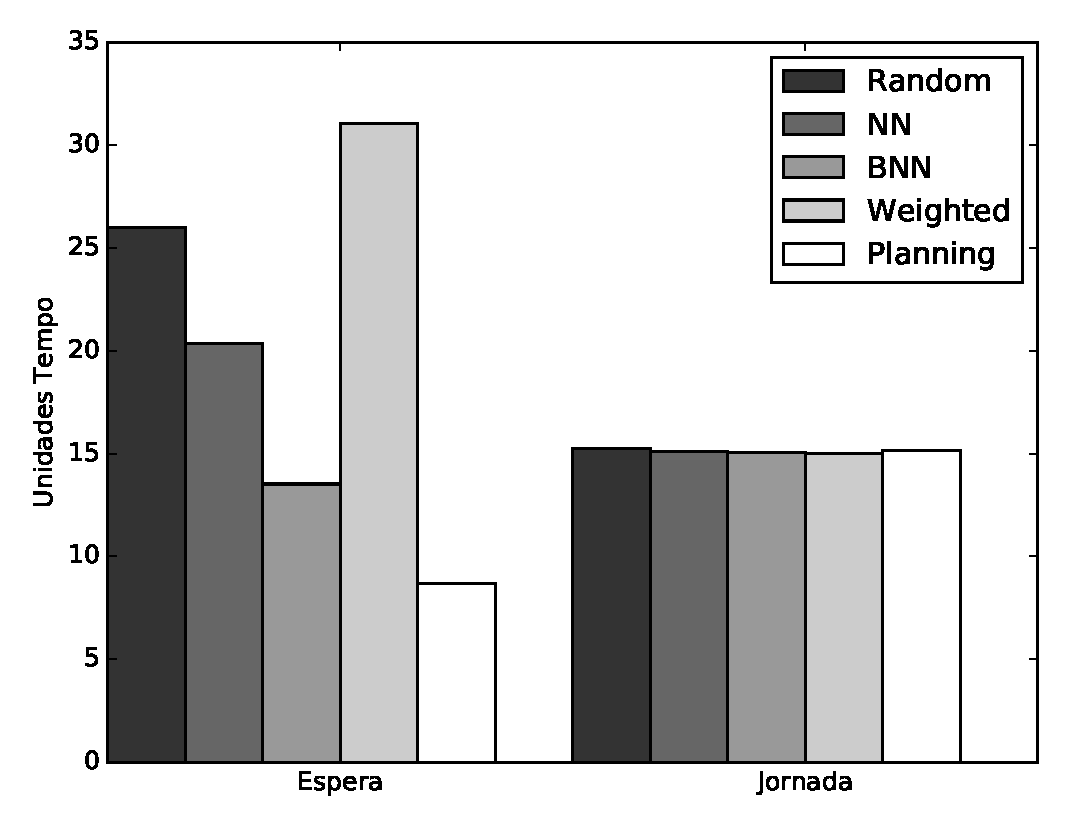
\includegraphics[scale=0.6]{img/high-rise-average-times-chart}
  \caption{Gráfico de resultados para o cenário \textit{High-rise}.}
  \label{fig:result:average:high-rise}
\end{figure}

\section{Cenário \textit{Skyscraper}}
A Listagem \ref{lst:config:skyscraper} exibe um excerto do arquivo de
configuração que define o cenário \textit{Skyscraper}. A Tabela
\ref{tab:results:skyscraper} mostra os resultados\footnote{Destacados encontram-
se os melhores resultados obtidos para cada métrica.} obtidos após a simulação.

\begin{listing}[htb!]
  \centering
    \begin{minted}[linenos,fontsize=\small]{yaml}
  # ...
  - name: Skyscraper
    duration: 43200 # unidades de tempo
    scheduler: [ 0, 1 ]
    planningHorizon: 2
    cost_function: [ 0, 1, 2, 3 ]
    seed: NimatYvEnU9QeE3GkF4J
    elevators: 16
    capacity: 12
    floors: [ 150, 300, 450, 600, 150, 300, 450, 600, 150, 300, 450, 450, 150,
              300, 450, 600, 150, 300, 450, 600, 150, 300, 450, 450, 150, 300,
              450, 600, 150, 300, 450, 600, 150, 300, 450, 450, 300, 450, 450,
              450, 150, 300, 450, 600, 150, 300, 450, 600, 150, 300, 450, 450,
              150, 300, 450, 600, 150, 300, 450, 600, 150, 300, 450, 450, 150,
              300, 450, 600, 150, 300, 450, 600, 150, 300, 450, 450, 300, 450,
              450, 450, 150, 300, 450, 600, 150, 300, 450, 600, 150, 300, 450,
              450, 150, 300, 450, 600, 150, 300, 450, 600, 150, 300, 450, 450,
              150, 300, 450, 600, 150, 300, 450, 600, 150, 300, 450, 450, 300,
              450, 450, 450, 150, 300, 450, 600, 150, 300, 450, 600, 150, 300,
              450, 450, 150, 300, 450, 600, 150, 300, 450, 600, 150, 300, 450,
              450, 150, 300, 450, 600, 150, 300, 450, 600, 150, 300, 450, 450,
              300, 450, 450, 450, 450, 450, 450 ]
  # ...
    \end{minted}
  \caption{Configuração do cenário \textit{Skyscraper}.}
  \label{lst:config:skyscraper}
\end{listing}

\begin{table}[htb!]
\centering
\caption{Resultados para o cenário \textit{Skyscraper}.}
\label{tab:results:skyscraper}
\begin{tabular}{|l|r|r|r|r|r|r|}
\hline
\multicolumn{1}{|c|}{\textbf{}} & \multicolumn{3}{c|}{\textbf{Tempo de Espera}} & \multicolumn{3}{c|}{\textbf{Tempo de Jornada}} \\ \hline
\textbf{Estratégia} & \multicolumn{1}{c|}{\textit{Médio}} & \multicolumn{1}{c|}{\textit{Desvio}} & \multicolumn{1}{c|}{\textit{Total}} & \multicolumn{1}{c|}{\textit{Médio}} & \multicolumn{1}{c|}{\textit{Desvio}} & \multicolumn{1}{c|}{\textit{Total}} \\ \hline
\textit{Simple / Random}   & 442.2165       & 1775.3156       & 10538904       & 54.7816        & 389.3520       & 1305554        \\ \hline
\textit{Simple / NN}       & 343.5988       & 1426.3821       &  8188647       & 54.9789        & 291.2258       & 1310258        \\ \hline
\textit{Simple / BNN}      & 287.1803       & 1137.2342       &  6844080       & 55.0124        & 235.4007       & 1311056        \\ \hline
\textit{Simple / Weighted} & 293.8791       & 1018.5118       &  7003726       & \green 54.6163 & 242.3278       & \green 1301616 \\ \hline
\textit{Planning}          & \green 78.3855 & \green 230.8554 & \green 1868084 & 60.1728        & \green 48.8070 & 1434038        \\ \hline
\end{tabular}
\end{table}

Novamente, o crescimento do cenário - tanto em número de andares como em número
de clientes - resultou em uma melhoria significativa dos resultados obtidos pelo
\textit{planning}. No maior de todos os cenários simulados, obteve-se
\textit{tempo de espera médio} e \textit{desvio padrão} $72.71\%$ e $79.70\%$
superiores em relação ao segundo colocado, respectivamente.

\begin{figure}[htb!]
  \centering
  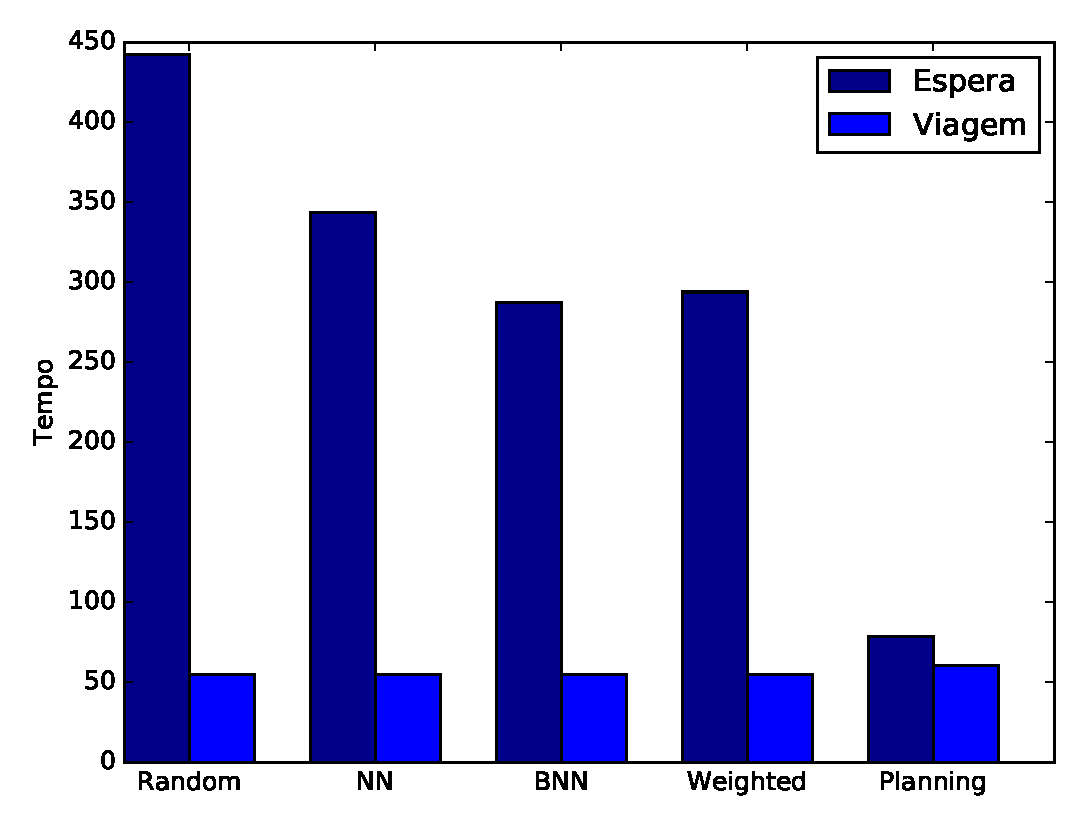
\includegraphics[scale=0.6]{img/skyscraper-average-times-chart}
  \caption{Gráfico de resultados para o cenário \textit{Skyscraper}.}
  \label{fig:result:average:skyscraper}
\end{figure}

\section{Tempo de Decisão do \textit{Planning}}

A Tabela~\ref{table:results:time} contém estatísticas do tempo de execução do
algoritmo, i.e. o tempo necessário para tomar a decisão de qual elevador deve
atender um cliente. Esta estatística é importante pois fornece uma medida do
impacto pela aplicação da solução em um sistema real: o agendamento seria
executado a cada vez que um botão de chamada é pressionado em todo o prédio.

\begin{table}[htb!]
\centering
\caption{Tempo de decisão do \textit{planning}.}
\label{table:results:time}
\begin{tabular}{|c|c|c|c|}
\hline
                 & \textbf{Low-rise} & \textbf{High-rise} & \textbf{Skyscraper} \\ \hline
\textit{Mínimo}  & 0.2220 ms         & 0.002097 s         & 0.03882 s           \\ \hline
\textit{Mediana} & 0.2900 ms         & 0.031623 s         & 2.35068 s           \\ \hline
\textit{Média}   & 0.4137 ms         & 0.043263 s         & 2.12851 s           \\ \hline
\textit{Máximo}  & 3.6810 ms         & 0.358810 s         & 4.99215 s           \\ \hline
\end{tabular}
\end{table}

Observa-se que o tempo é muito reduzido para os cenários \textit{Low-rise} e
\textit{High-rise}, causando quase nenhum impacto. Já para o cenário
\textit{Skyscraper} os números parecem ruins a primeira vista. Porém, ao
considerar os resultados para tempo de espera, um tempo médio de 2.13 segundos e
um máximo de 4.99 segundos não causam prejuízo significativo. Por estas razões,
o desempenho do \textit{planning} foi considerado plenamente satisfatório.

\section{Anexos}

Para fins de referência, tem-se a seguir os gráficos de tempo de espera médio
por andar, divididos por cenário.

\begin{figure}[htb!]
  \centering
  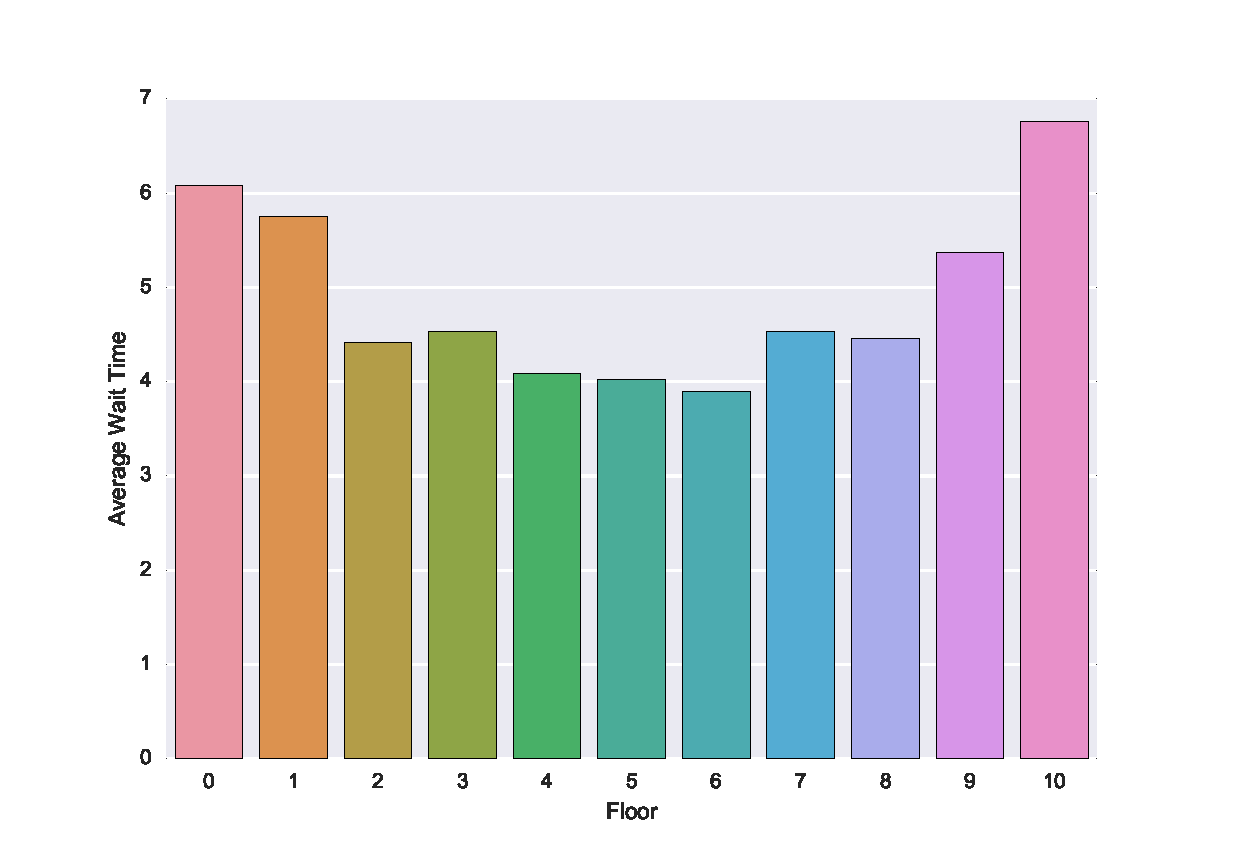
\includegraphics[scale=0.8]{img/results/Low-rise/1_Simple_Random/averageWaitTime}
  \caption{Tempo médio de espera para Random no cenário Low-rise}
  \label{fig:result:low-rise:avgwt:random}
\end{figure}

\begin{figure}[htb!]
  \centering
  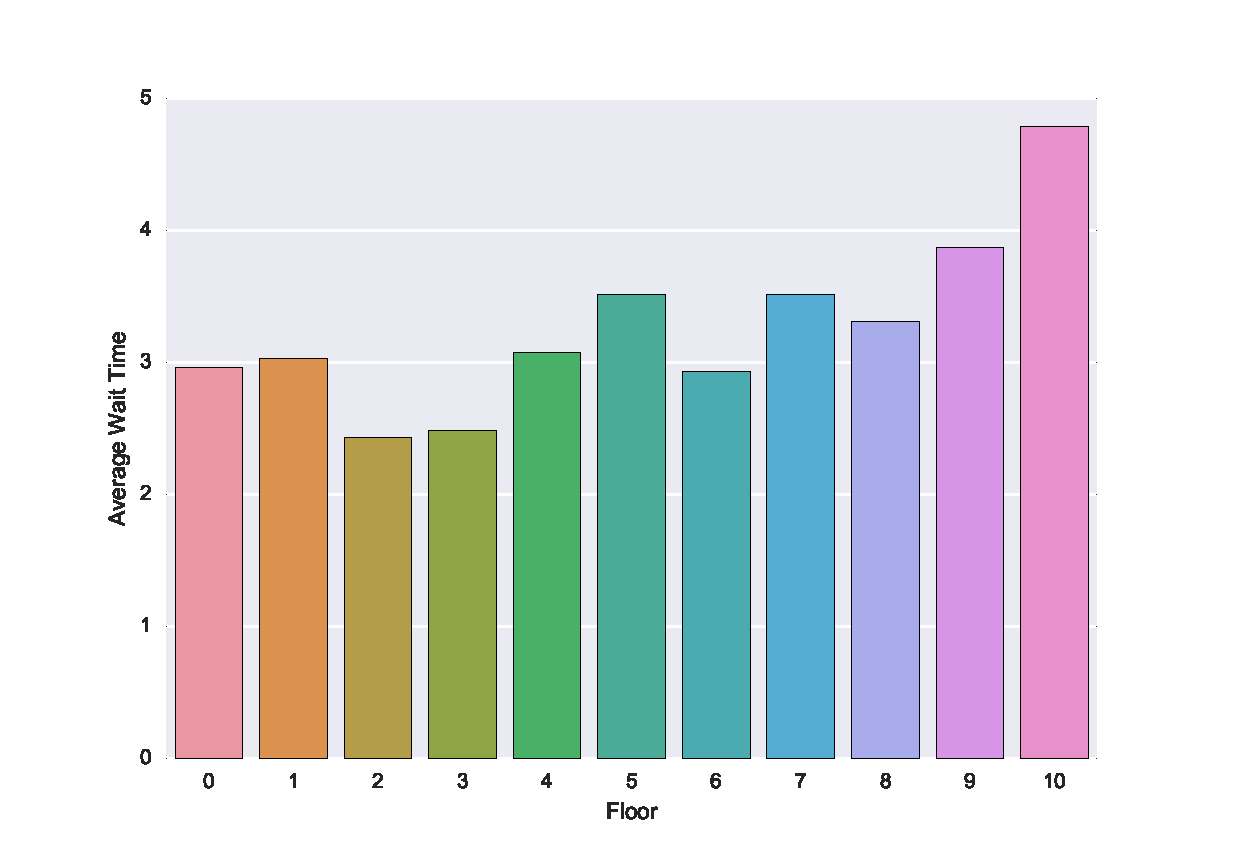
\includegraphics[scale=0.8]{img/results/Low-rise/2_Simple_NearestNeighbour/averageWaitTime}
  \caption{Tempo médio de espera para Nearest Neighbour no cenário Low-rise}
  \label{fig:result:low-rise:avgwt:nn}
\end{figure}

\begin{figure}[htb!]
  \centering
  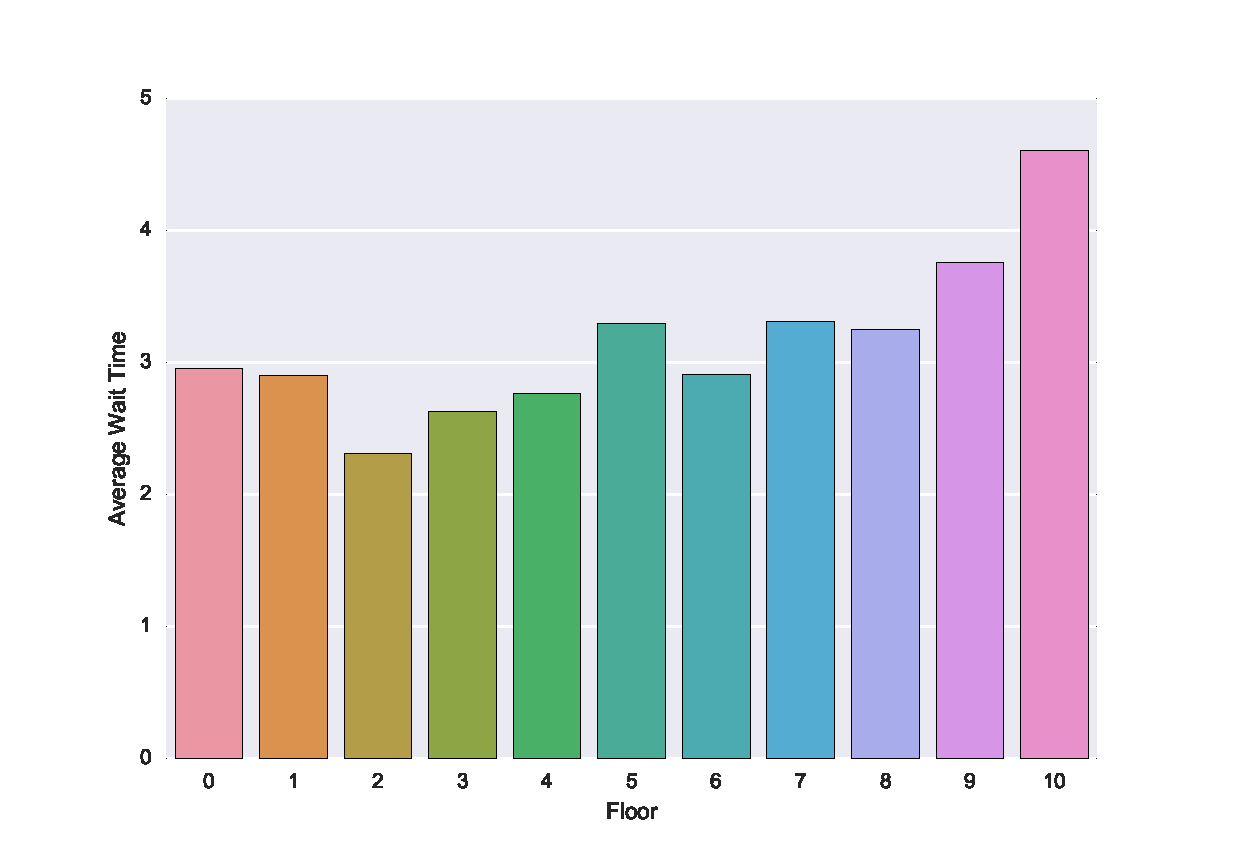
\includegraphics[scale=0.8]{img/results/Low-rise/3_Simple_BetterNearestNeighbour/averageWaitTime}
  \caption{Tempo médio de espera para Better Nearest Neighbour no cenário Low-rise}
  \label{fig:result:low-rise:avgwt:bnn}
\end{figure}

\begin{figure}[htb!]
  \centering
  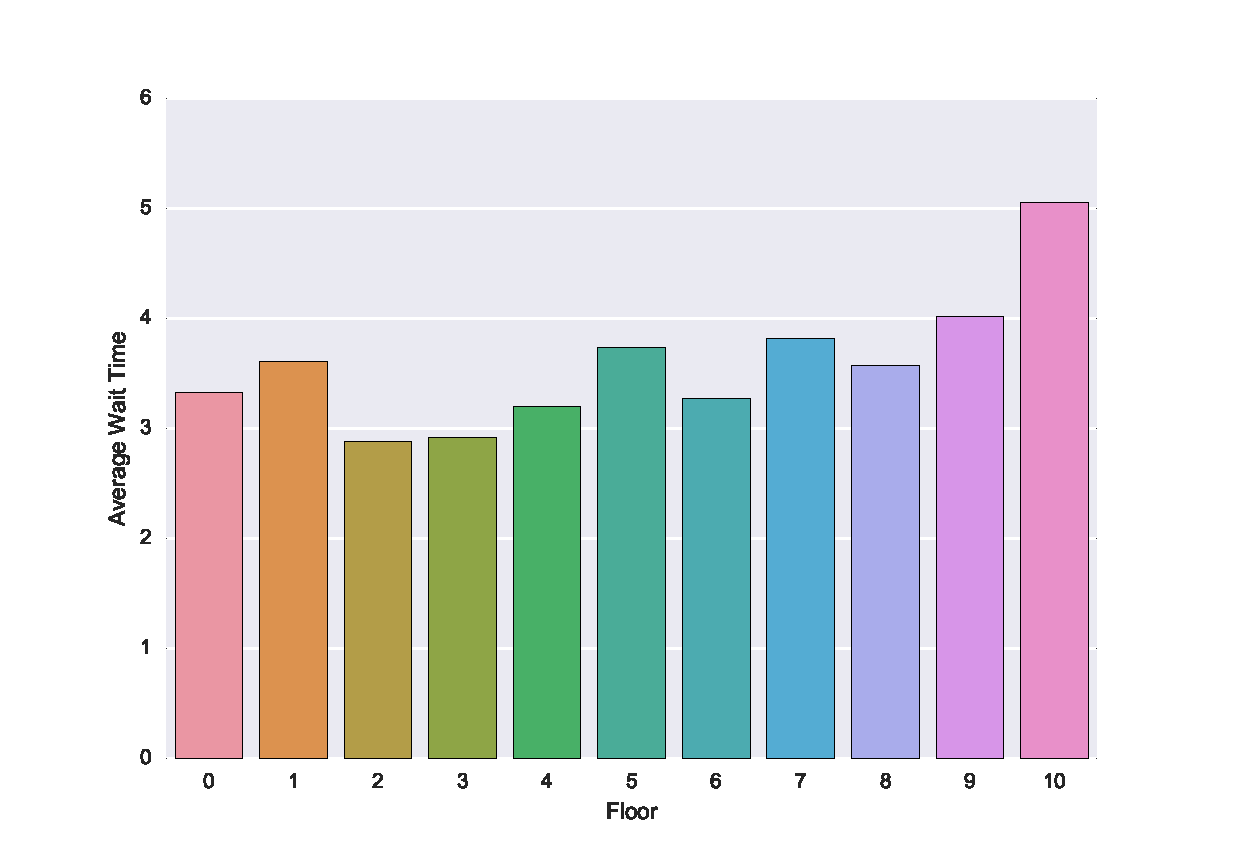
\includegraphics[scale=0.8]{img/results/Low-rise/4_Simple_Weighted/averageWaitTime}
  \caption{Tempo médio de espera para Weighted no cenário Low-rise}
  \label{fig:result:low-rise:avgwt:weighted}
\end{figure}

\begin{figure}[htb!]
  \centering
  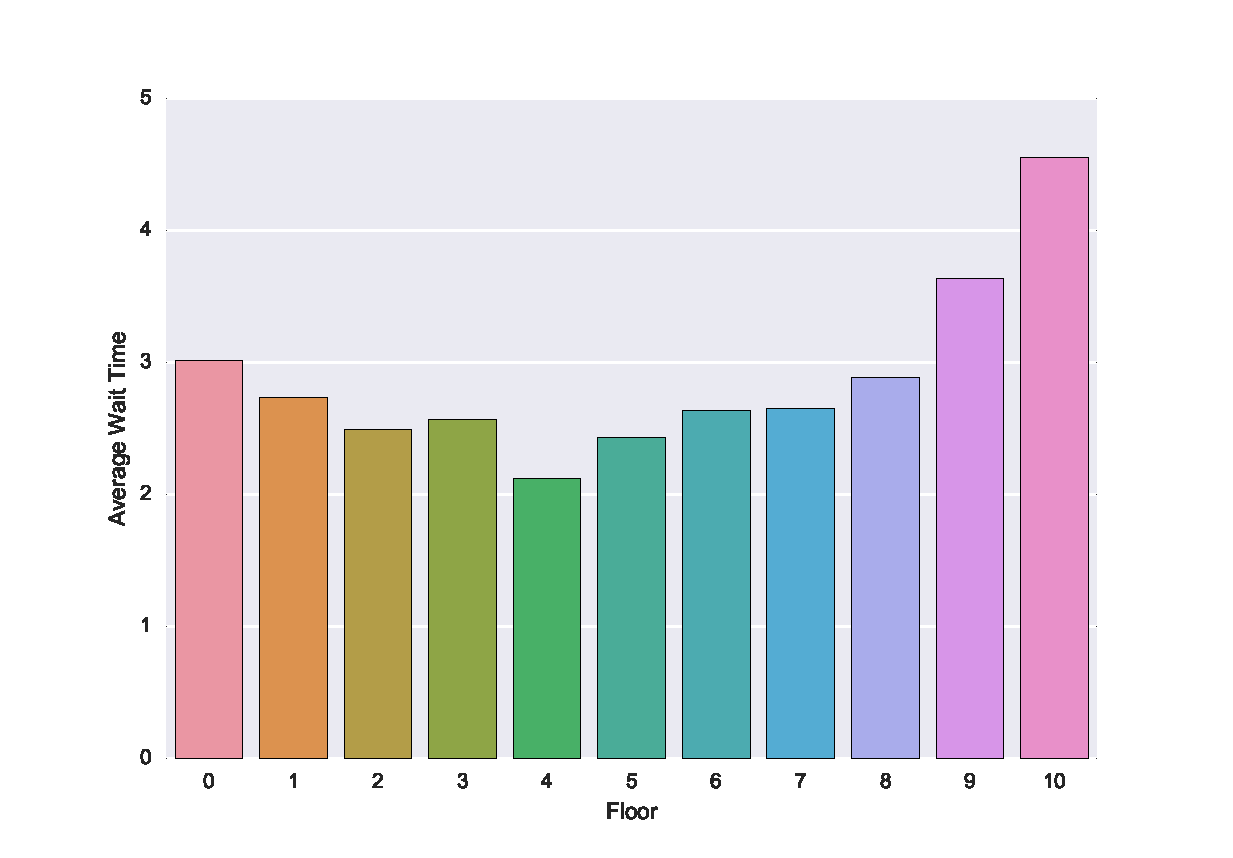
\includegraphics[scale=0.8]{img/results/Low-rise/5_Planning_Random/averageWaitTime}
  \caption{Tempo médio de espera para Planning no cenário Low-rise}
  \label{fig:result:low-rise:avgwt:planning}
\end{figure}

\begin{figure}[htb!]
  \centering
  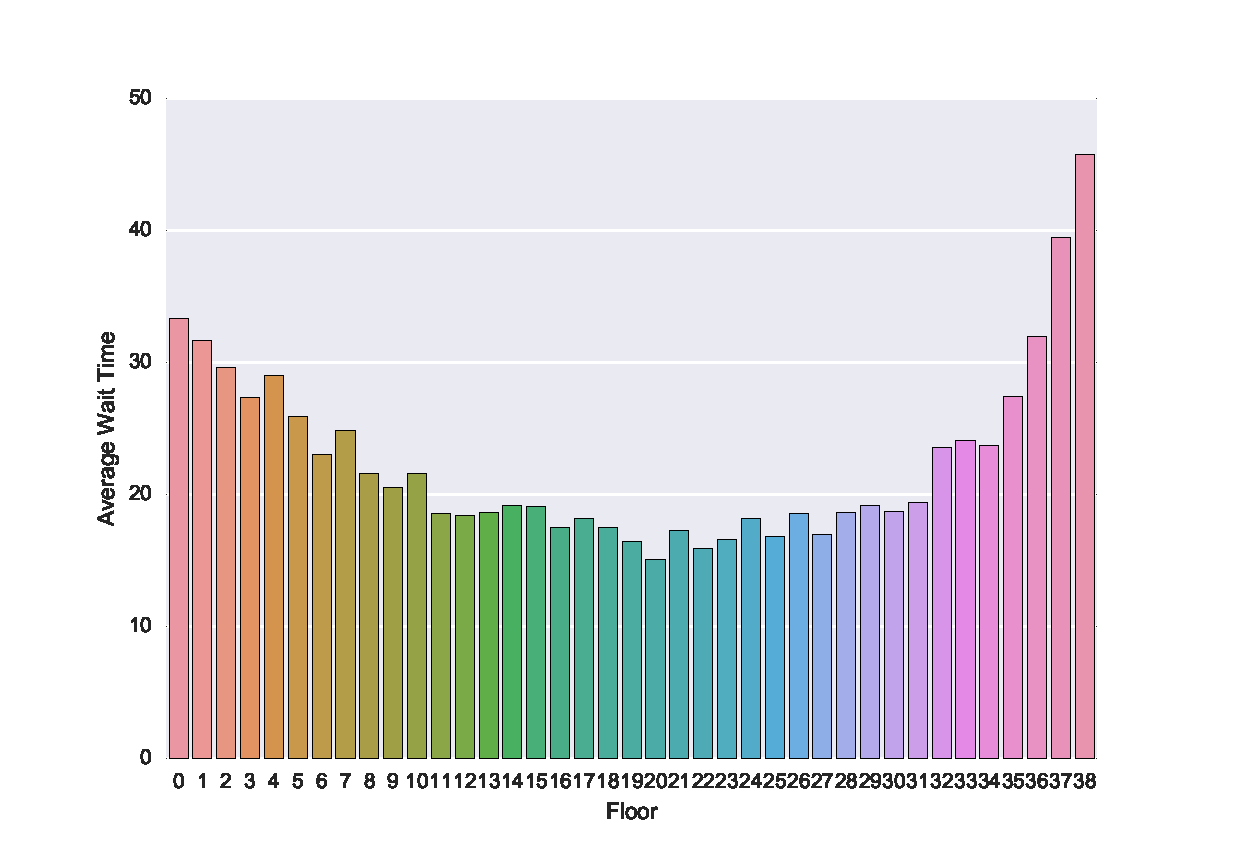
\includegraphics[scale=0.8]{img/results/High-rise/1_Simple_Random/averageWaitTime}
  \caption{Tempo médio de espera para Random no cenário High-rise}
  \label{fig:result:high-rise:avgwt:random}
\end{figure}

\begin{figure}[htb!]
  \centering
  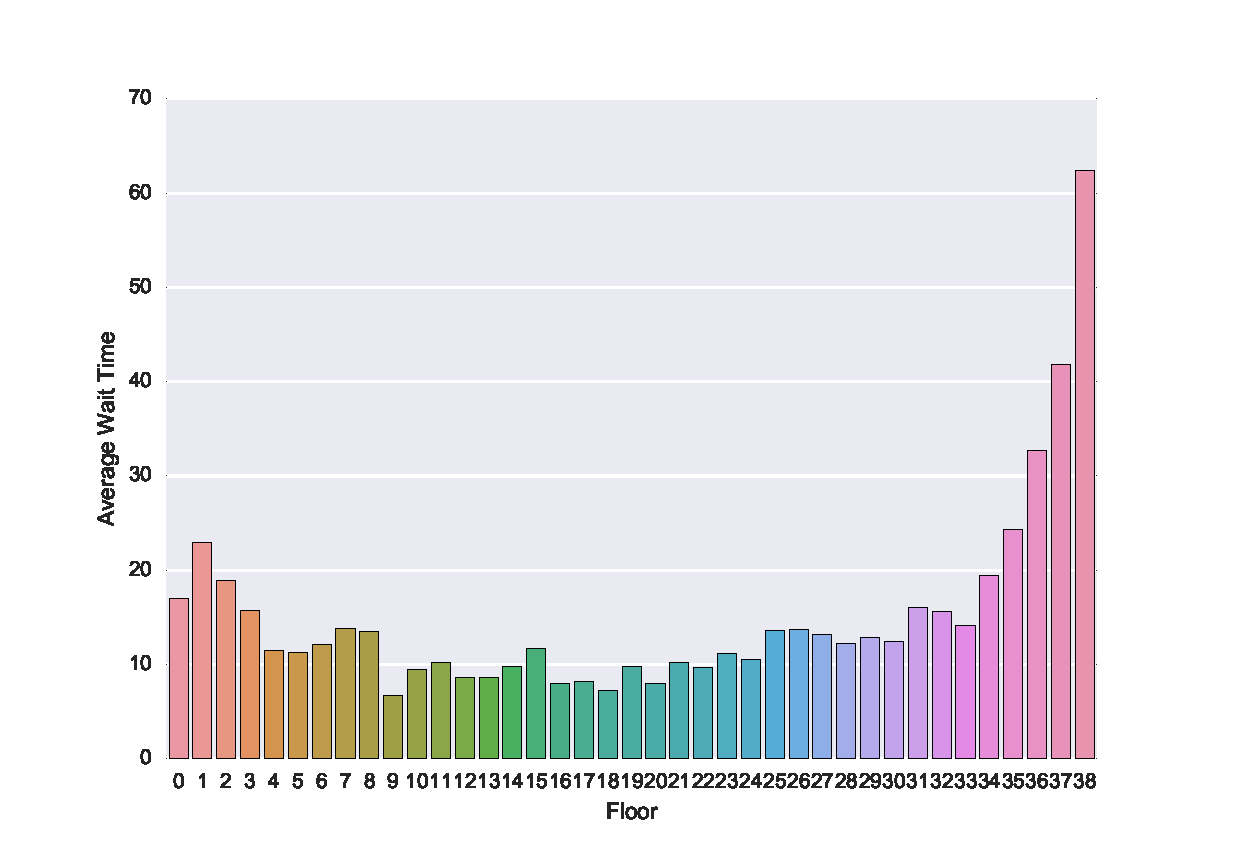
\includegraphics[scale=0.8]{img/results/High-rise/2_Simple_NearestNeighbour/averageWaitTime}
  \caption{Tempo médio de espera para Nearest Neighbour no cenário High-rise}
  \label{fig:result:high-rise:avgwt:nn}
\end{figure}

\begin{figure}[htb!]
  \centering
  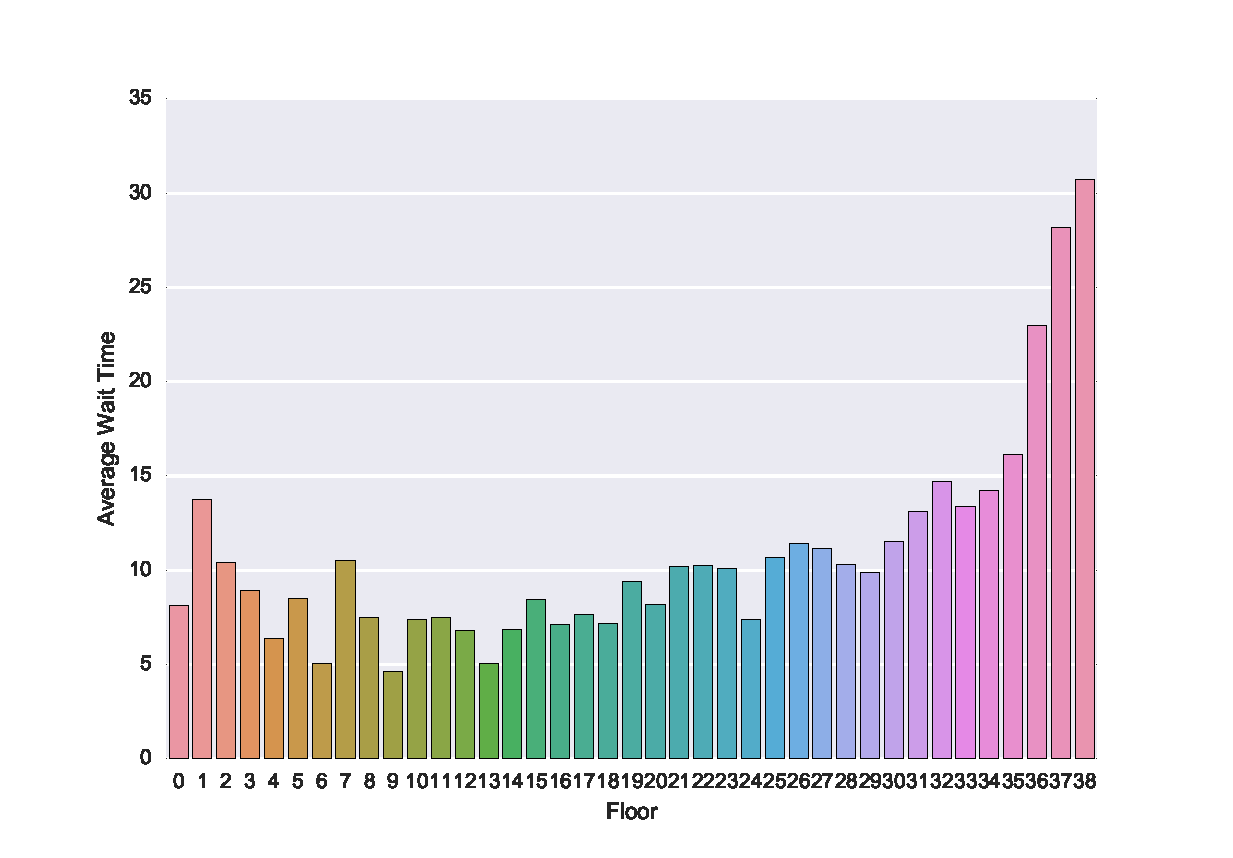
\includegraphics[scale=0.8]{img/results/High-rise/3_Simple_BetterNearestNeighbour/averageWaitTime}
  \caption{Tempo médio de espera para Better Nearest Neighbour no cenário High-rise}
  \label{fig:result:high-rise:avgwt:bnn}
\end{figure}

\begin{figure}[htb!]
  \centering
  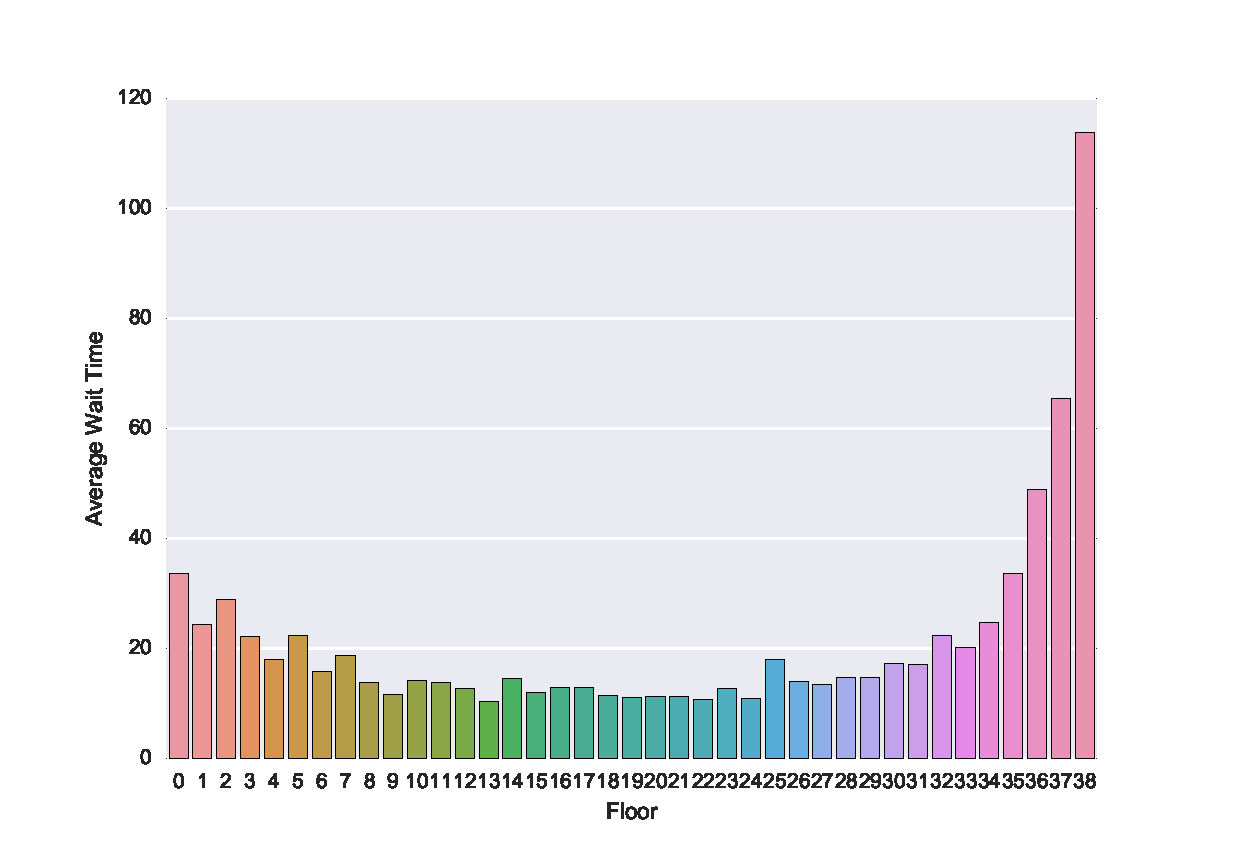
\includegraphics[scale=0.8]{img/results/High-rise/4_Simple_Weighted/averageWaitTime}
  \caption{Tempo médio de espera para Weighted no cenário High-rise}
  \label{fig:result:high-rise:avgwt:weighted}
\end{figure}

\begin{figure}[htb!]
  \centering
  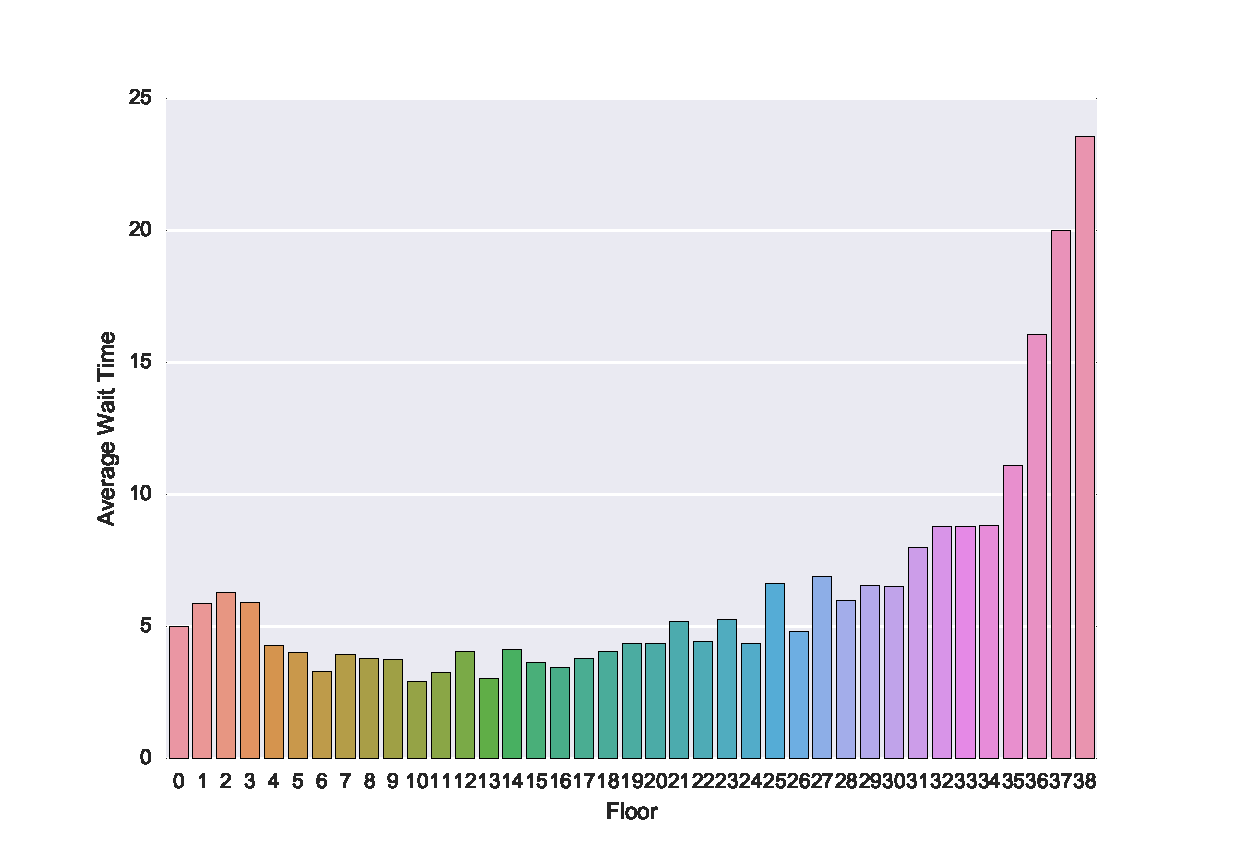
\includegraphics[scale=0.8]{img/results/High-rise/5_Planning_Random/averageWaitTime}
  \caption{Tempo médio de espera para Planning no cenário High-rise}
  \label{fig:result:high-rise:avgwt:planning}
\end{figure}

\begin{figure}[htb!]
  \centering
  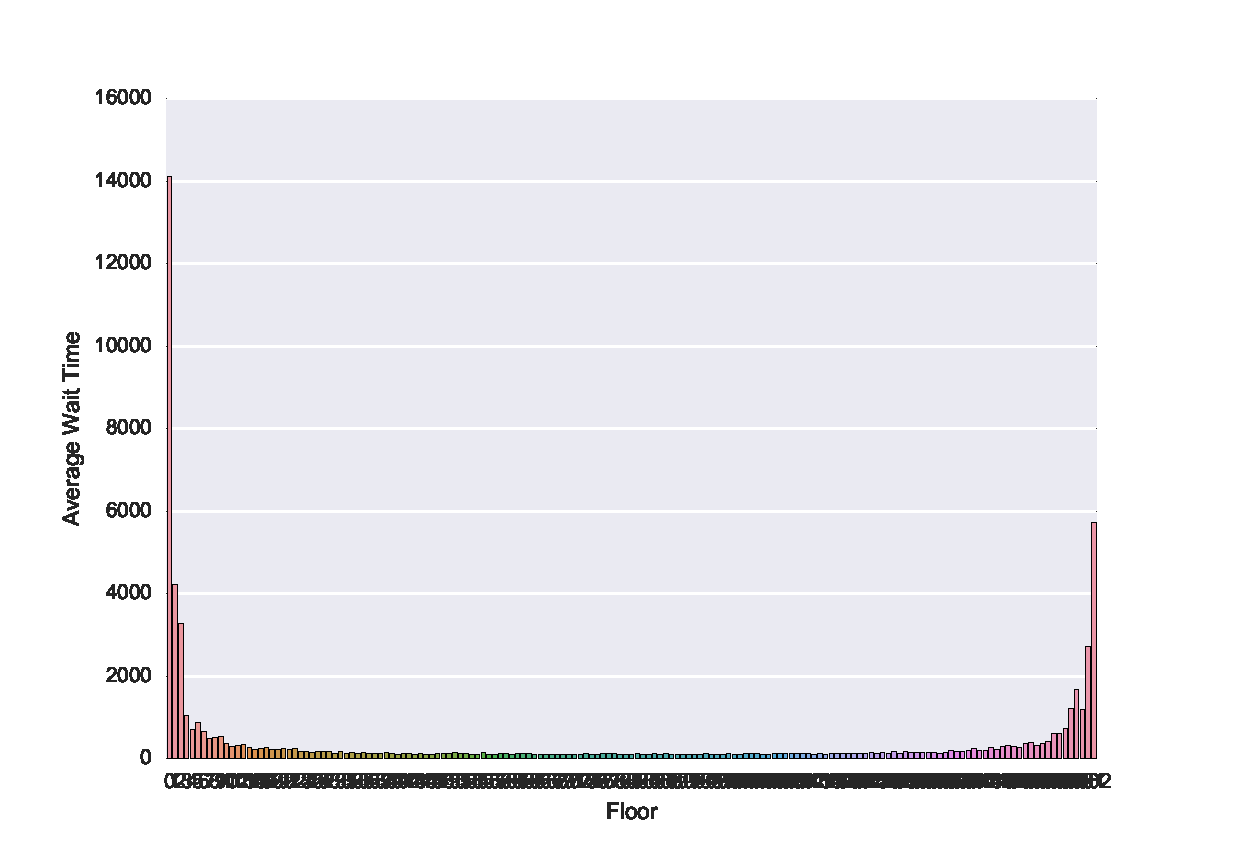
\includegraphics[scale=0.8]{img/results/Skyscraper/1_Simple_Random/averageWaitTime}
  \caption{Tempo médio de espera para Random no cenário Skyscraper}
  \label{fig:result:skyscraper:avgwt:random}
\end{figure}

\begin{figure}[htb!]
  \centering
  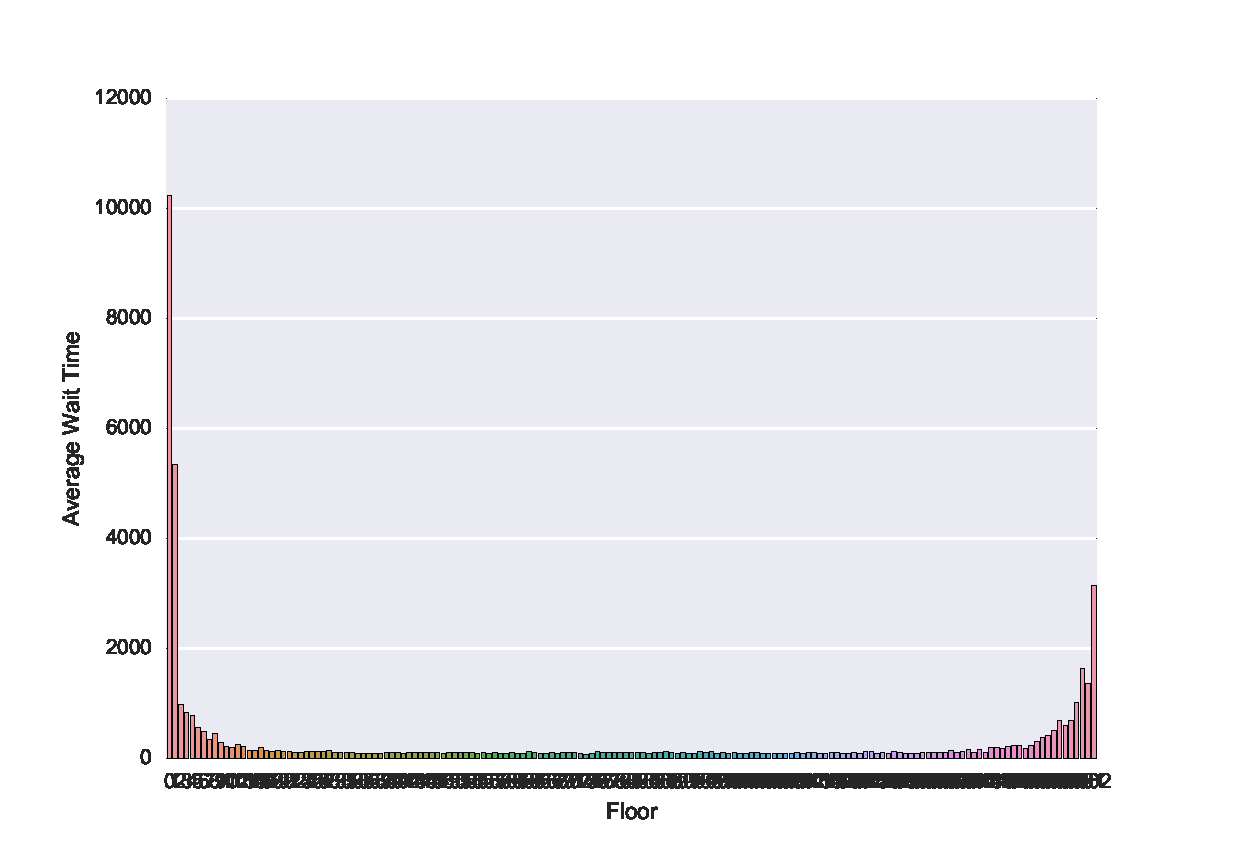
\includegraphics[scale=0.8]{img/results/Skyscraper/2_Simple_NearestNeighbour/averageWaitTime}
  \caption{Tempo médio de espera para Nearest Neighbour no cenário Skyscraper}
  \label{fig:result:skyscraper:avgwt:nn}
\end{figure}

\begin{figure}[htb!]
  \centering
  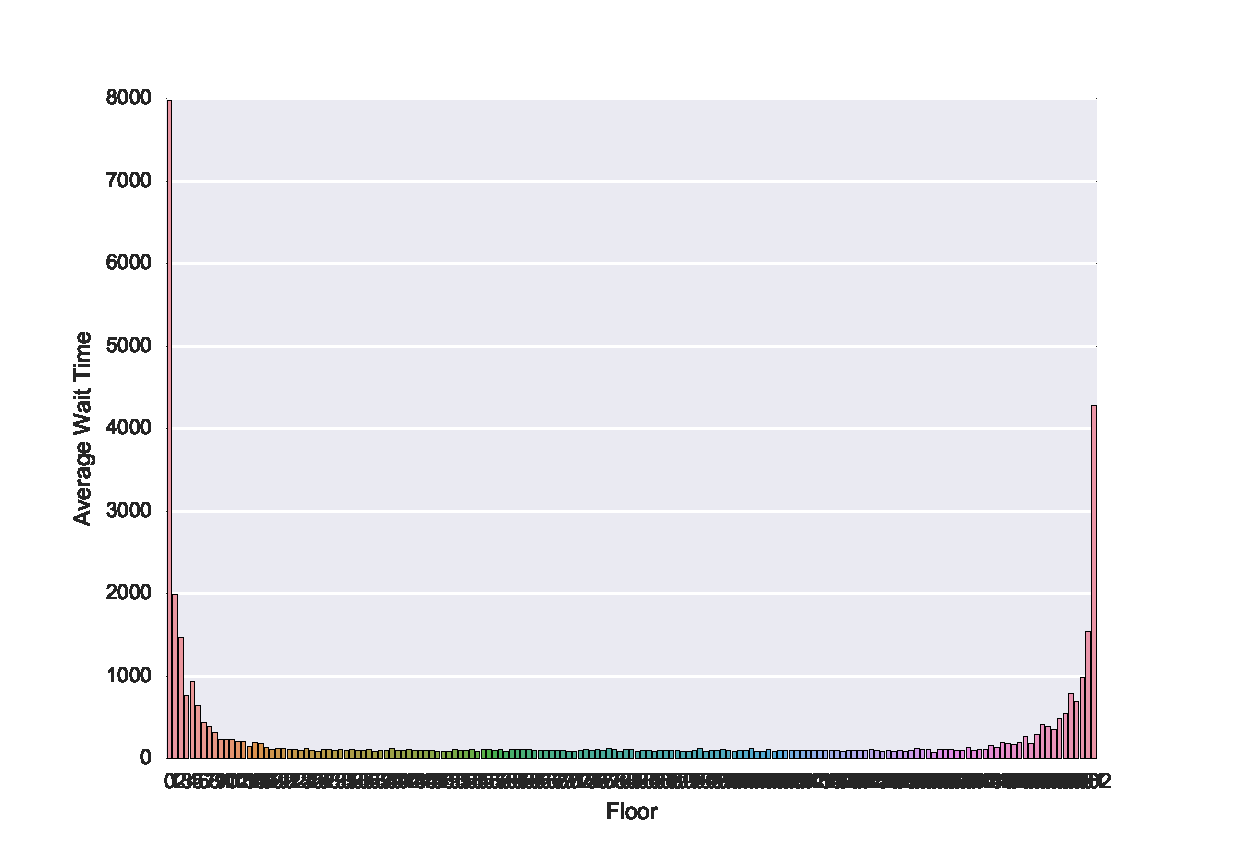
\includegraphics[scale=0.8]{img/results/Skyscraper/3_Simple_BetterNearestNeighbour/averageWaitTime}
  \caption{Tempo médio de espera para Better Nearest Neighbour no cenário Skyscraper}
  \label{fig:result:skyscraper:avgwt:bnn}
\end{figure}

\begin{figure}[htb!]
  \centering
  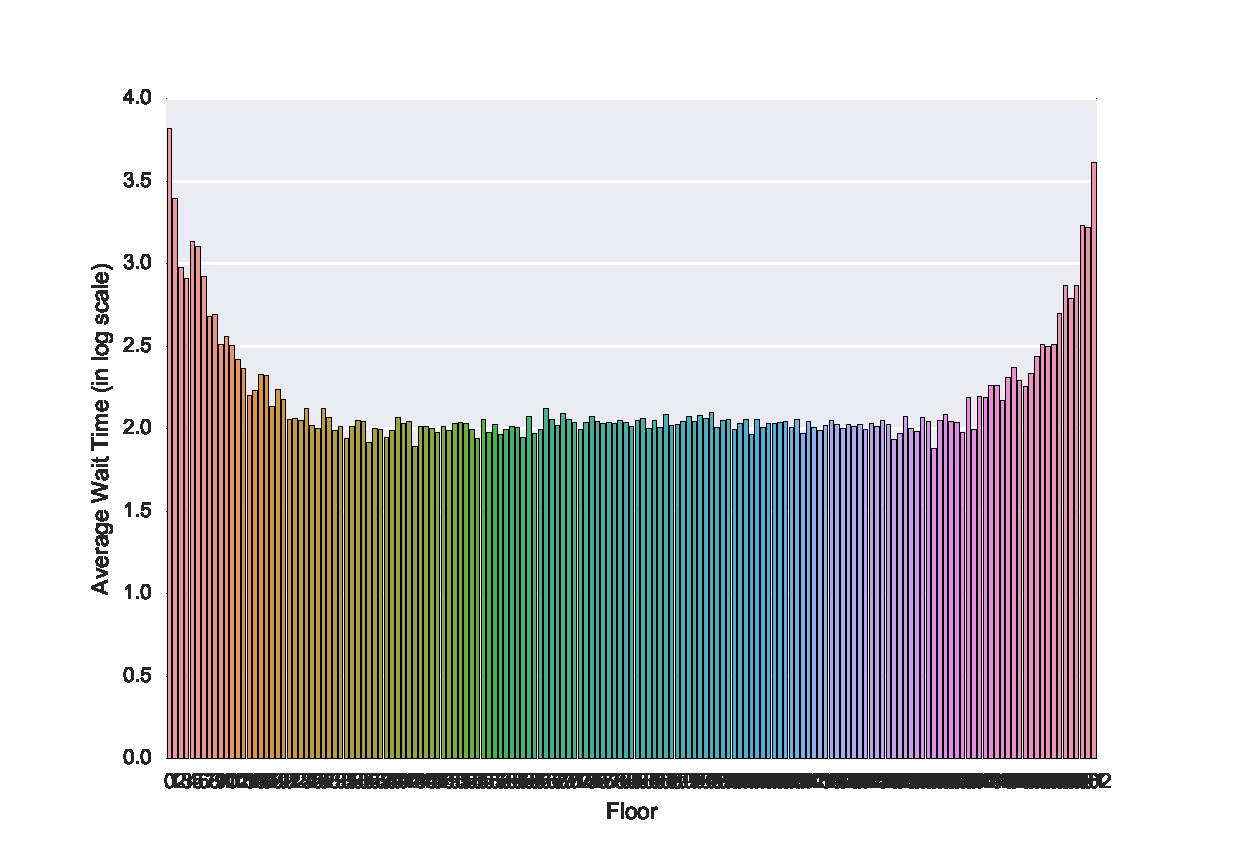
\includegraphics[scale=0.8]{img/results/Skyscraper/4_Simple_Weighted/averageWaitTime}
  \caption{Tempo médio de espera para Weighted no cenário Skyscraper}
  \label{fig:result:skyscraper:avgwt:weighted}
\end{figure}

\begin{figure}[htb!]
  \centering
  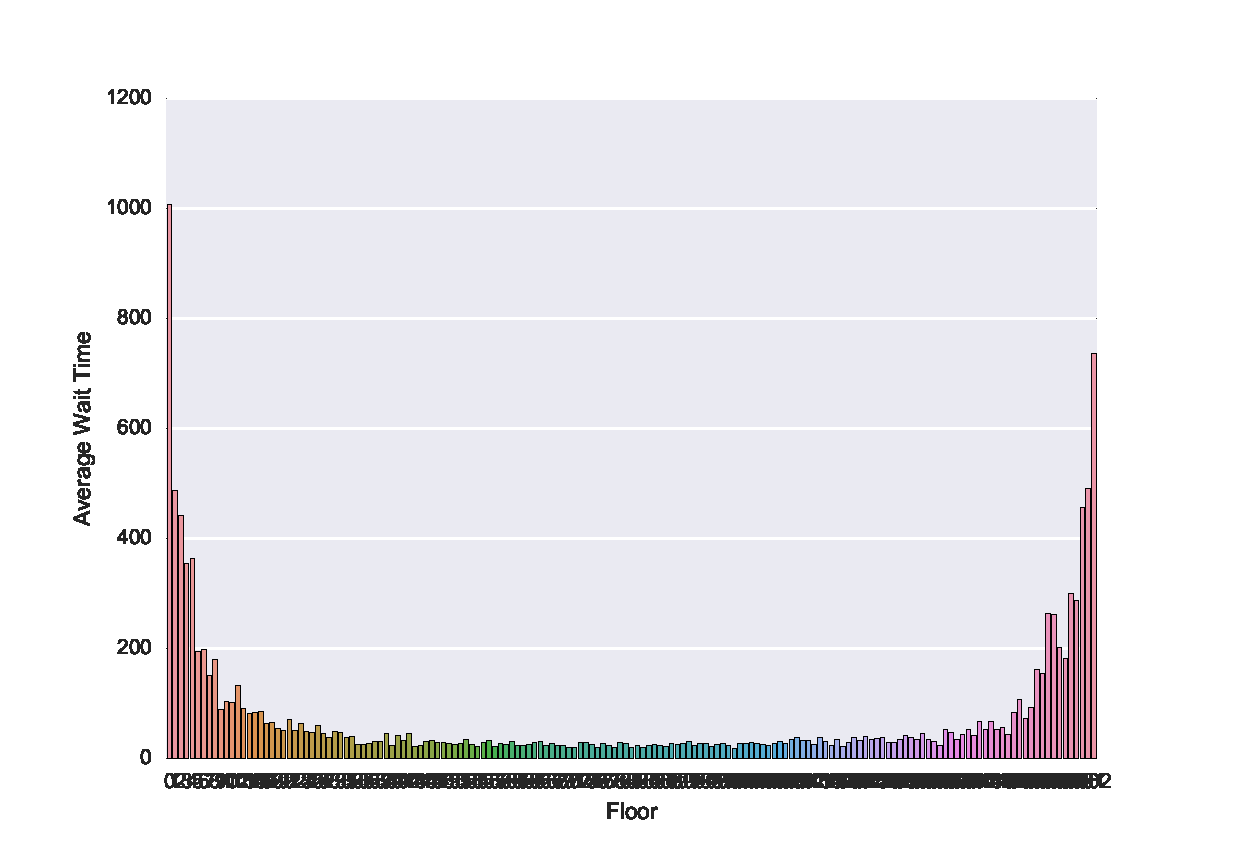
\includegraphics[scale=0.8]{img/results/Skyscraper/5_Planning_Random/averageWaitTime}
  \caption{Tempo médio de espera para Planning no cenário Skyscraper}
  \label{fig:result:skyscraper:avgwt:planning}
\end{figure}